\chapstart
\section{THIẾT KẾ GIAO DIỆN}
\subsection{Định hướng thiết kế}
Giao diện BroomSharing sử dụng xanh lục và xanh ngọc trên nền trắng, xám nhẹ; thống nhất tiêu đề, trường nhập, thẻ phòng và nút chính. Nội dung được mở dần từ danh sách đến chi tiết, thời gian và chi phí.

Các hình trong chương là prototype ban đầu trên Figma. Chúng thể hiện bố cục và hướng tương tác; giao diện hiện thực được trình bày ở Chương 5 và quy trình sử dụng ở Chương 6. Những lựa chọn hợp đồng hoặc phương thức đăng nhập trong prototype không đồng nghĩa đã được tích hợp vào ứng dụng.

\subsection{Giao diện người thuê}
\subsubsection{Đăng nhập và đăng ký}
Hình~\ref{fig:ch3-auth} nhóm trường tài khoản, mật khẩu và liên hệ theo thứ tự nhập; nút gửi biểu mẫu có màu nhấn, còn liên kết đăng ký và quên mật khẩu đặt riêng. Biểu tượng mật khẩu hỗ trợ kiểm tra nội dung nhập. Thiết kế dành phản hồi cho dữ liệu thiếu, sai định dạng hoặc xác thực không thành công, đồng thời giữ phần thông tin còn hợp lệ khi sửa lỗi.

\begin{figure}[H]\centering
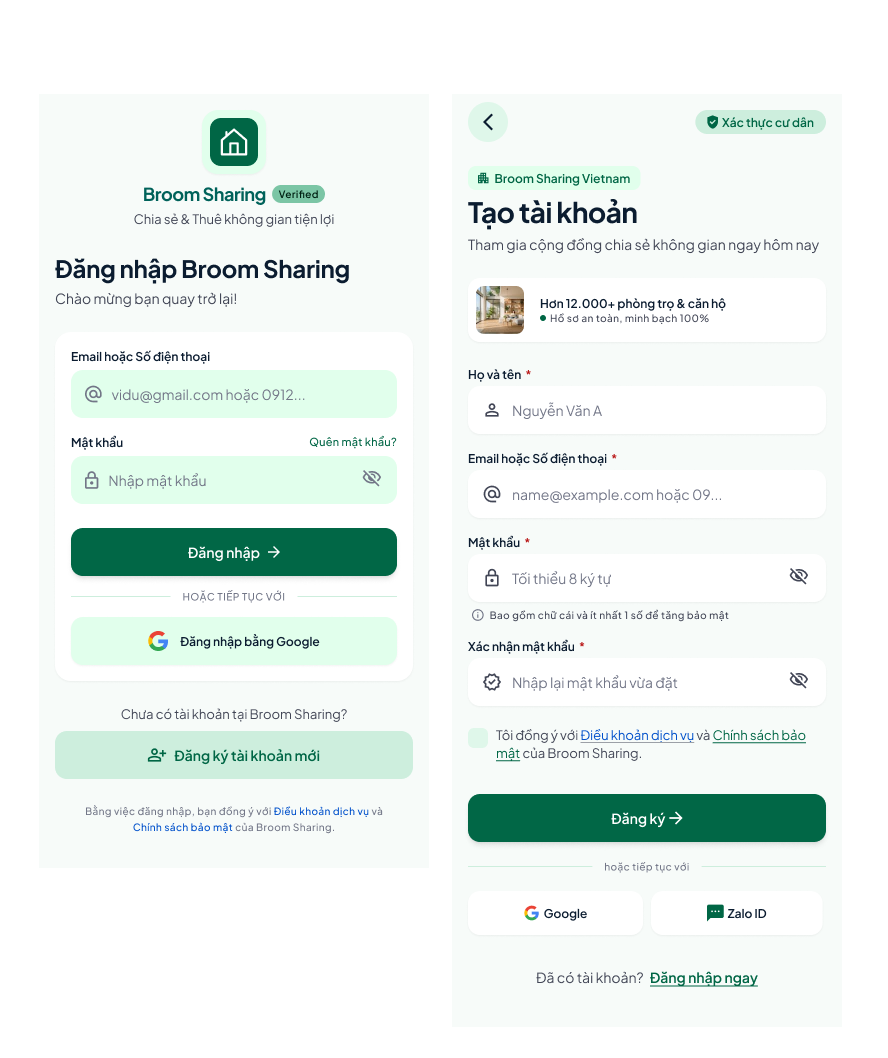
\includegraphics[width=0.9\textwidth,height=0.43\textheight,keepaspectratio]{chapter3/auth-design.png}
\caption{Thiết kế biểu mẫu đăng nhập và đăng ký tài khoản.}\label{fig:ch3-auth}
\end{figure}
\clearpage

\subsubsection{Trang chủ và chi tiết không gian}
Trang chủ trong Hình~\ref{fig:ch3-home} đặt tìm kiếm, danh mục và thẻ không gian theo thứ bậc; ảnh, tên, khu vực và đơn vị giá hỗ trợ so sánh nhanh. Thanh điều hướng đáy duy trì lối vào các nhóm chức năng. Danh sách hiện thực sử dụng RecyclerView để tái sử dụng View khi hiển thị \parencite{android_recycler}.

Chi tiết phòng tại Hình~\ref{fig:ch3-detail} mở rộng bộ ảnh, sức chứa, tiện ích, vị trí và thông tin Host thành các khối có thể cuộn. Yêu thích, nhắn tin, chỉ đường và đặt thuê gắn với phòng đang xem. Đơn vị giá đặt sát số tiền để phân biệt thuê giờ và kỳ thuê cố định.

\begin{figure}[H]\centering
\begin{minipage}[t]{0.31\textwidth}\centering
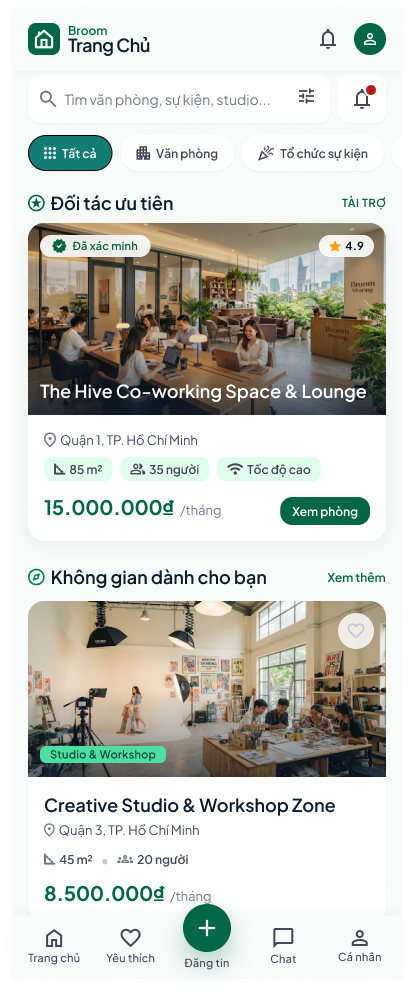
\includegraphics[width=\linewidth,height=0.53\textheight,keepaspectratio]{chapter3/home-design.png}
\caption{Thiết kế Trang chủ.}\label{fig:ch3-home}
\end{minipage}\hfill
\begin{minipage}[t]{0.65\textwidth}\centering
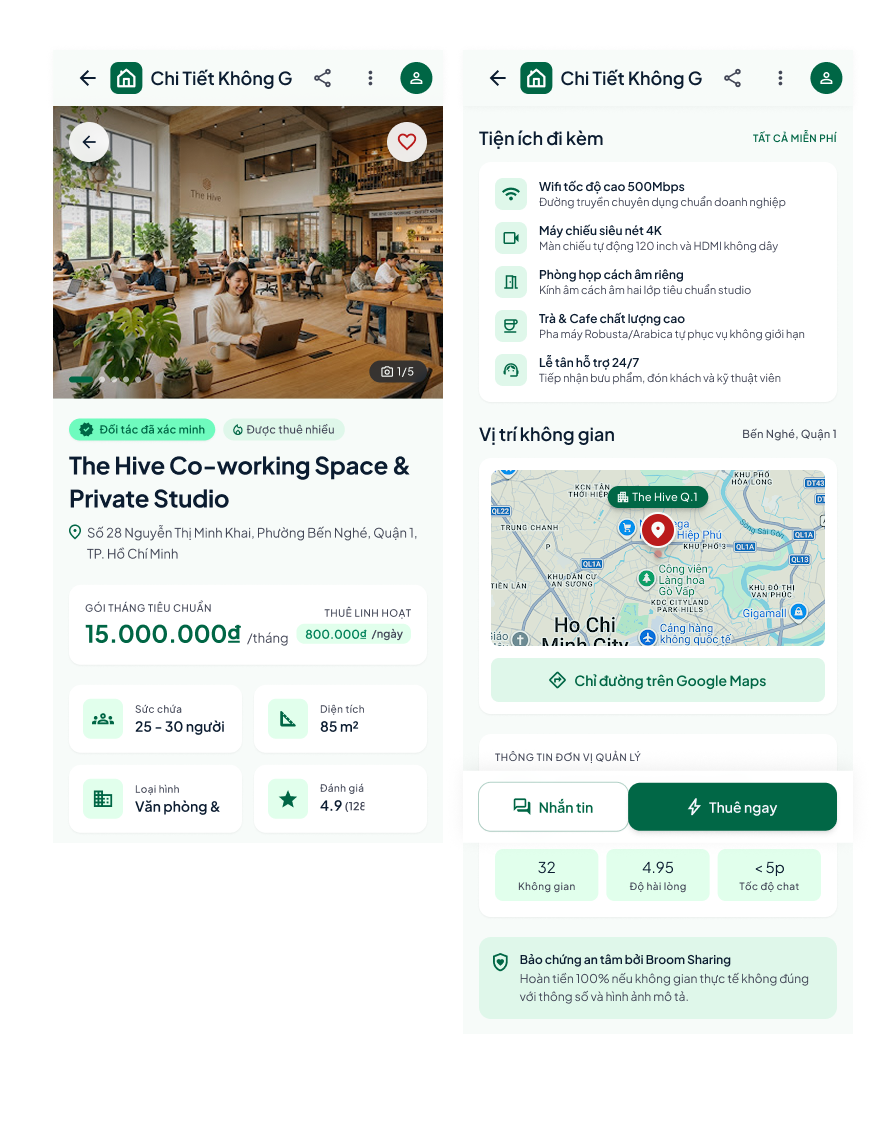
\includegraphics[trim=0 88 0 0,clip,width=\linewidth,height=0.53\textheight,keepaspectratio]{chapter3/detail-design.png}
\caption{Thiết kế thông tin chi tiết không gian.}\label{fig:ch3-detail}
\end{minipage}
\end{figure}
\clearpage

\subsubsection{Đặt chỗ và tương tác}
Hình~\ref{fig:app-booking-design} tập hợp phòng, thời gian, liên hệ và chi phí trước khi gửi yêu cầu. Tổng tiền và nút chính nằm cuối tiến trình; thay đổi thời gian phải cập nhật phần chi phí liên quan. Các lựa chọn hợp đồng, bảo chứng và tiền cọc trong hình thuộc phương án ban đầu, còn quy trình hiện thực tuân theo chính sách thanh toán của Chương 2.

\begin{figure}[H]\centering
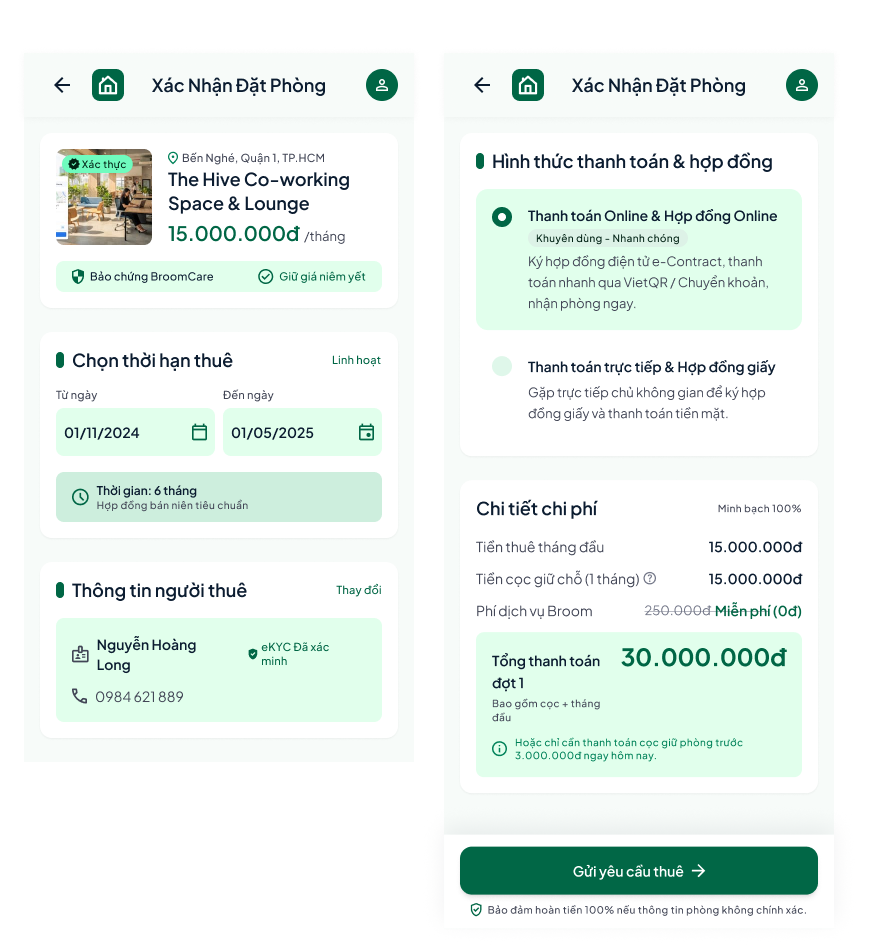
\includegraphics[width=\textwidth,height=0.56\textheight,keepaspectratio]{chapter3/booking-design.png}
\caption{Prototype xác nhận thông tin và chi phí đặt phòng.}\label{fig:app-booking-design}
\end{figure}

Hồ sơ phân nhóm thông tin cá nhân, ảnh đại diện, yêu thích và lịch sử. Hội thoại giữ ngữ cảnh phòng; hộp cập nhật dẫn về đúng lượt thuê liên quan. Đánh giá gắn với lượt đã xác nhận sử dụng, trong khi báo cáo vi phạm có biểu mẫu riêng gửi Admin.
\clearpage

\subsection{Giao diện chủ không gian}
Biểu mẫu Host tại Hình~\ref{fig:ch3-host} chia ba bước: thông tin cơ bản, giá và lịch, hình ảnh và điều kiện sử dụng. Thanh tiến trình cùng nút quay lại, tiếp tục cho phép kiểm tra nội dung trước khi gửi; dữ liệu cần được giữ khi chuyển giữa các bước. Vùng ảnh phân biệt tệp đã chọn, đang tải và lỗi tải.

\begin{figure}[H]\centering
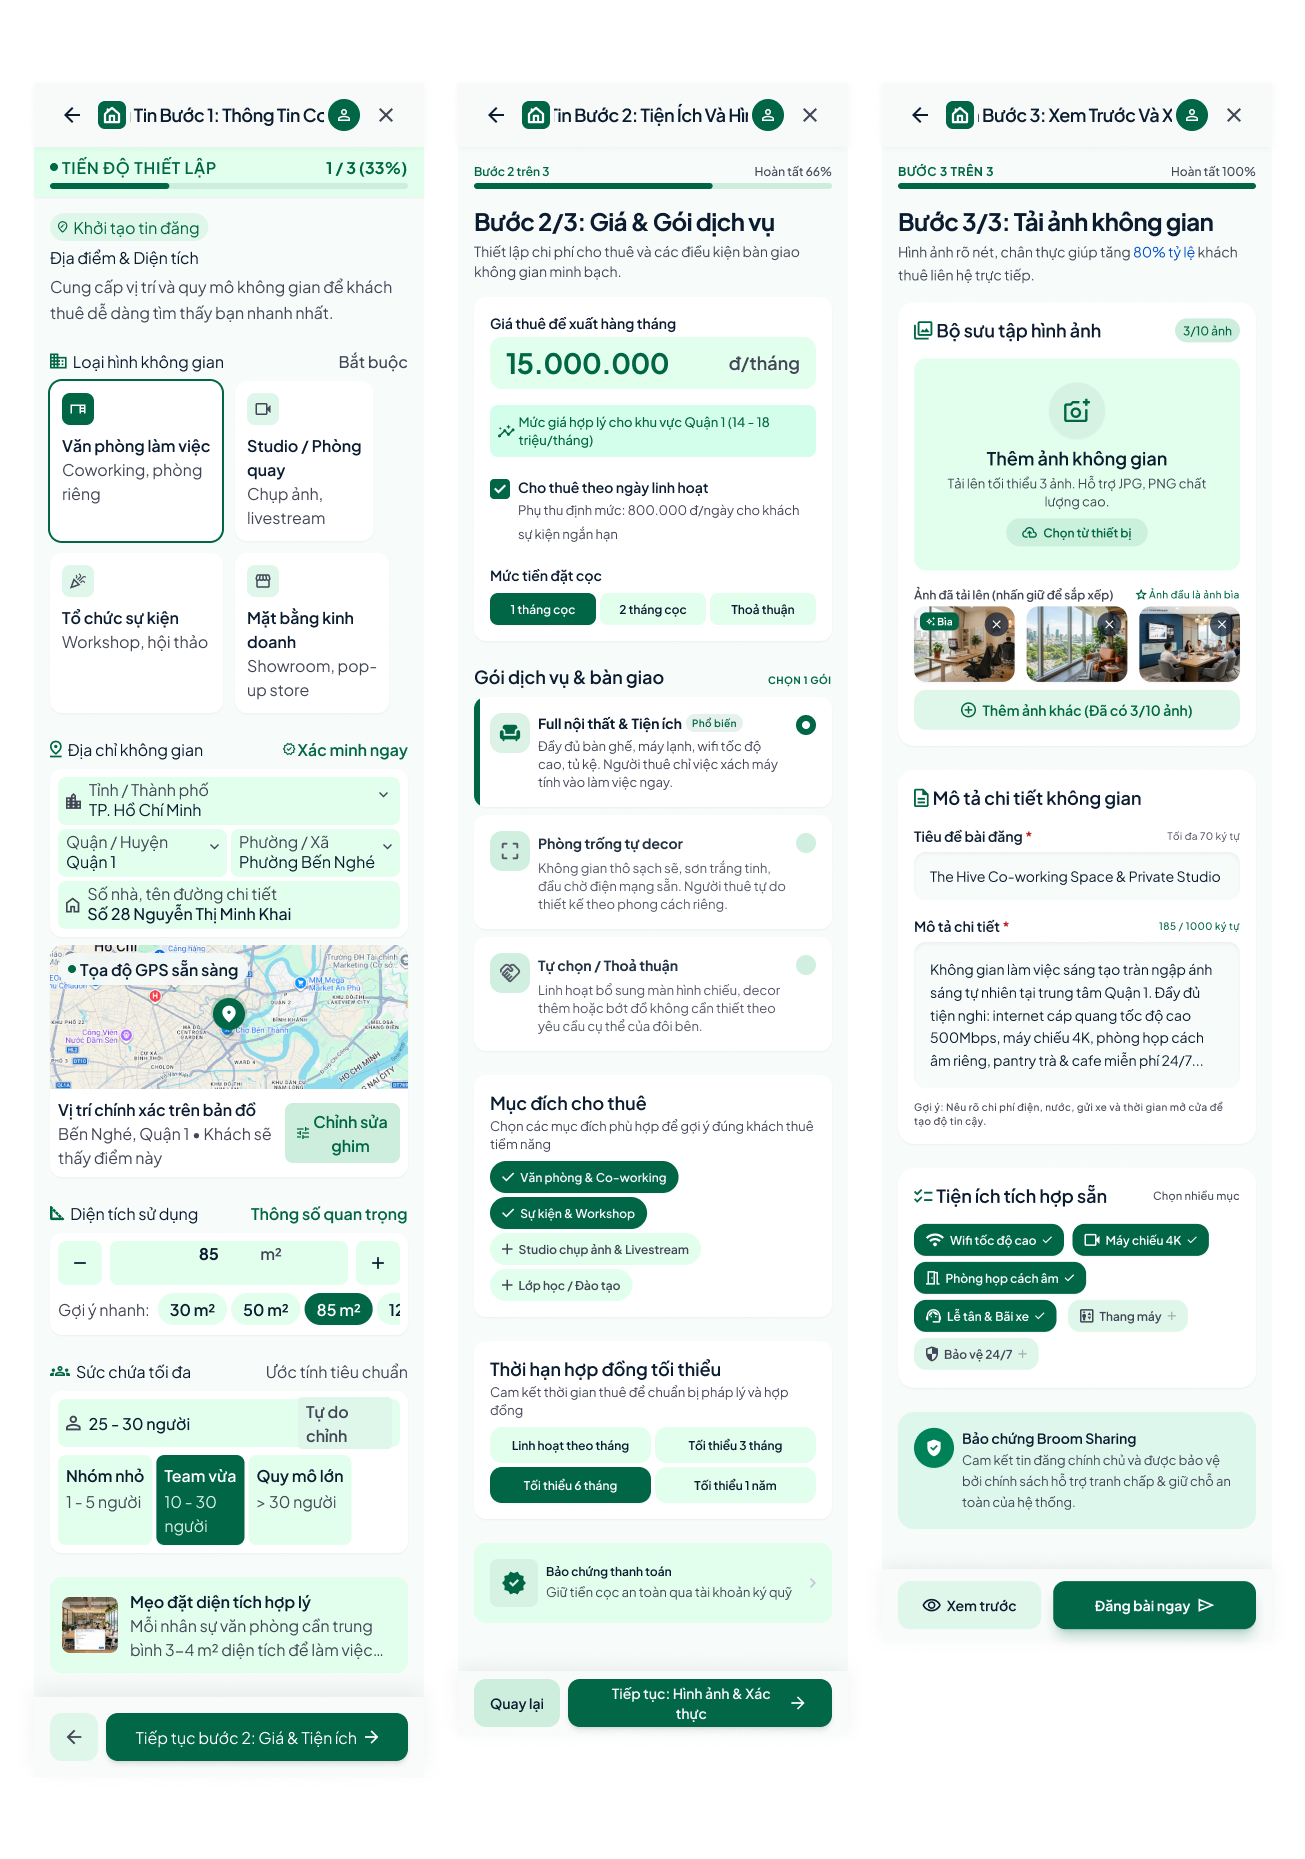
\includegraphics[width=\textwidth,height=0.48\textheight,keepaspectratio]{chapter3/host-design.png}
\caption{Prototype ba bước nhập thông tin và đăng không gian.}\label{fig:ch3-host}
\end{figure}

Khu vực quản lý tập trung phòng, booking và lịch. Nhãn chờ duyệt khác nhãn tạm ngừng; các thao tác nhận phòng, hoàn tất, không đến hoặc hủy được hiển thị theo trạng thái. Hành động ảnh hưởng lượt thuê cần xác định đúng đối tượng và yêu cầu lý do khi phù hợp.

\subsection{Giao diện quản trị viên}
Admin được tổ chức thành tổng quan, xét duyệt, quản lý và báo cáo. Bộ lọc giúp chọn loại hồ sơ, còn quyết định chấp thuận hoặc từ chối gắn với thẻ đang xem. Đơn cấp quyền Host độc lập với minh chứng vị trí, hình ảnh. Prototype trong Hình~\ref{fig:app-admin-design} ở Phụ lục B minh họa cách nhóm thông tin và thao tác này; các con số chỉ phục vụ thiết kế bố cục.
